% !TeX program = xelatex
\documentclass[9pt]{beamer}
\usepackage{xcolor}
\definecolor{orange}{HTML}{EF767A}
\definecolor{red}{HTML}{AC454A}
\definecolor{brown}{HTML}{EAD296}
\definecolor{darkgrey}{HTML}{313630}
\definecolor{cornflower}{HTML}{247BA0}
\definecolor{sienna}{HTML}{6C464F}
\usefonttheme{professionalfonts} % using non standard fonts for beamer
\usefonttheme{serif} % default family is serif
\usepackage{fontspec}
\usepackage{setspace}
\usepackage{natbib}
\usepackage{animate}
\usepackage{graphicx}
%\usepackage[T1]{fontenc}

\bibliographystyle{abbrv}
%\setmainfont{Liberation Serif}
%\setmainfont{Liberation Serif}
\setmainfont{Comfortaa}
%\usepackage[T1]{fontenc}

\setbeamercolor{frametitle}{bg=orange,fg=white}
\setbeamercolor{author in head/foot}{bg=orange,fg=white}

%\setbeamerfont{page number}{size=\Huge}

%\setbeamertemplate{itemize itemjpegs}[circle]
\useinnertheme{circles}
\setbeamercolor{palette primary}{bg=orange,fg=white}
%\setbeamercolor{palette secondary}{bg=red,fg=white}
\setbeamertemplate{itemize item}{\color{darkgrey}$\circ$}
\setbeamercolor{structure}{fg=red} % itemize, enumerate, etc

%\setbeamercolor{section in head/foot}{bg=red}
\setbeamercolor{title}{fg=orange} %, bg=brown
\setbeamercolor{author}{fg=darkgrey}
\setbeamercolor{institute}{fg=darkgrey}
\setbeamercolor{date}{fg=darkgrey}
%\setbeamercolor{normal text}{fg=darkgrey}
\makeatletter
\setbeamertemplate{headline}{%
	\usebeamercolor[bg]{frametitle}\rule{\textwidth}{1cm}
}
\setbeamerfont{title}{size=\LARGE}
\setbeamerfont{institute}{size=\normalsize}
\renewcommand*{\bibfont}{\scriptsize}


\setbeamertemplate{frametitle}{%
	\vskip-1cm%
	\begin{minipage}[c][\headheight][c]{\textwidth}%
		\usebeamerfont{frametitle}
		\strut\insertframetitle\par
		{%
			\ifx\insertframesubtitle\@empty%
			\else%
			{\usebeamerfont{framesubtitle}\usebeamercolor[fg]{framesubtitle}\strut\insertframesubtitle\par}%
			\fi
		}%      
		\vspace*{0.05cm}
	\end{minipage}%
	\vskip-0.1em
}
%\setbeamertemplate{footline}{%
%	\leavevmode%
%	\hbox{\begin{beamercolorbox}[wd=\paperwidth,ht=4.5ex,dp=3.125ex]{author in head/foot}%
%			\usebeamerfont{author in head/foot} bar
%	\end{beamercolorbox}}%
%	\vskip0pt%
%}
\makeatother


\title{Unsupervised Learning \\
	of Disentangled and Interpretable Representations from Sequential Data}
\author{Wei-Ning Hsu, Yu Zhang, and James Glass\\Talk by Stefan Wezel}
\institute{Seminar ML4S}

\date{\today}


%\setbeamertemplate{sidebar right}{}
%\setbeamertemplate{footline}{%
%	\hfill\usebeamertemplate***{navigation symbols}
%	\hspace{1cm}\insertframenumber{}}
\setbeamerfont{page number in head/foot}{size=\small}
    \setbeamertemplate{footline}{%
	\raisebox{5pt}{\makebox[\paperwidth]{\hfill\makebox[10pt]{\scriptsize\insertframenumber}}}}
\setbeamertemplate{navigation symbols}{}
%\onehalfspacing
\setstretch{1.3}
\begin{document}
	

\setbeamercolor{background canvas}{bg=white}
\setbeamercolor{normal text}{fg=darkgrey}
\usebeamercolor[fg]{normal text}
\begin{frame}[plain]
	\titlepage
\end{frame} 



\setbeamercolor{background canvas}{bg=white}
\setbeamercolor{normal text}{fg=darkgrey}
\usebeamercolor[fg]{normal text}
\setbeamertemplate{itemize item}{\color{darkgrey}$\circ$}
\begin{frame}
\frametitle{Overview}
%\framesubtitle{}
\begin{itemize}%\setlength\itemsep{1.5em}
	\item Introduction
	\item What are Disentangled Representations? (intuition)
	\item Why Disentangled Representations
	\item Formal Description of Disentangled Representations
	\item Disentanglement in the Context of the Paper
	\item The Factorized Hierarchical VAE Model
	\item Results
	%\item Other approaches and challenges
\end{itemize}
\end{frame} 



\setbeamercolor{background canvas}{bg=white}
\setbeamercolor{normal text}{fg=darkgrey}
\usebeamercolor[fg]{normal text}
\setbeamertemplate{itemize item}{\color{darkgrey}$\circ$}
\begin{frame}
\frametitle{Introduction}
\framesubtitle{Setting - Speech data}
\begin{itemize}%\setlength\itemsep{1.5em}
	\item Propose Sequential Factorized Hierarchical VAE (\textbf{FHVAE})
	%\item Learn factorized latent space
	\item Focus on speech data
	\begin{itemize}
		\item Sequence level (Speaker, ...) attributes
		\item Segment level (content, noise, ...) attributes
	\end{itemize}
	\item Reflect different temporal scales in latent space
\end{itemize}
\end{frame} 




\setbeamercolor{background canvas}{bg=white}
\setbeamercolor{normal text}{fg=darkgrey}
\usebeamercolor[fg]{normal text}
\setbeamertemplate{itemize item}{\color{darkgrey}$\circ$}
\begin{frame}
\frametitle{What is disentanglement?}
\framesubtitle{Intuition}
	\begin{itemize}%\setlength\itemsep{1.5em}
	\item Encode distinct generating factors in separate subsets of latent space dimensions
	%\item i.e. color as one subspace, translation, as another
	%\item The exact definition is often discussed, we will have a look at a proposed one
	\end{itemize}
%\animategraphics[autoplay,loop,width=\linewidth/2]{10}{disentangled_scene-}{0}{19}
\begin{figure}
	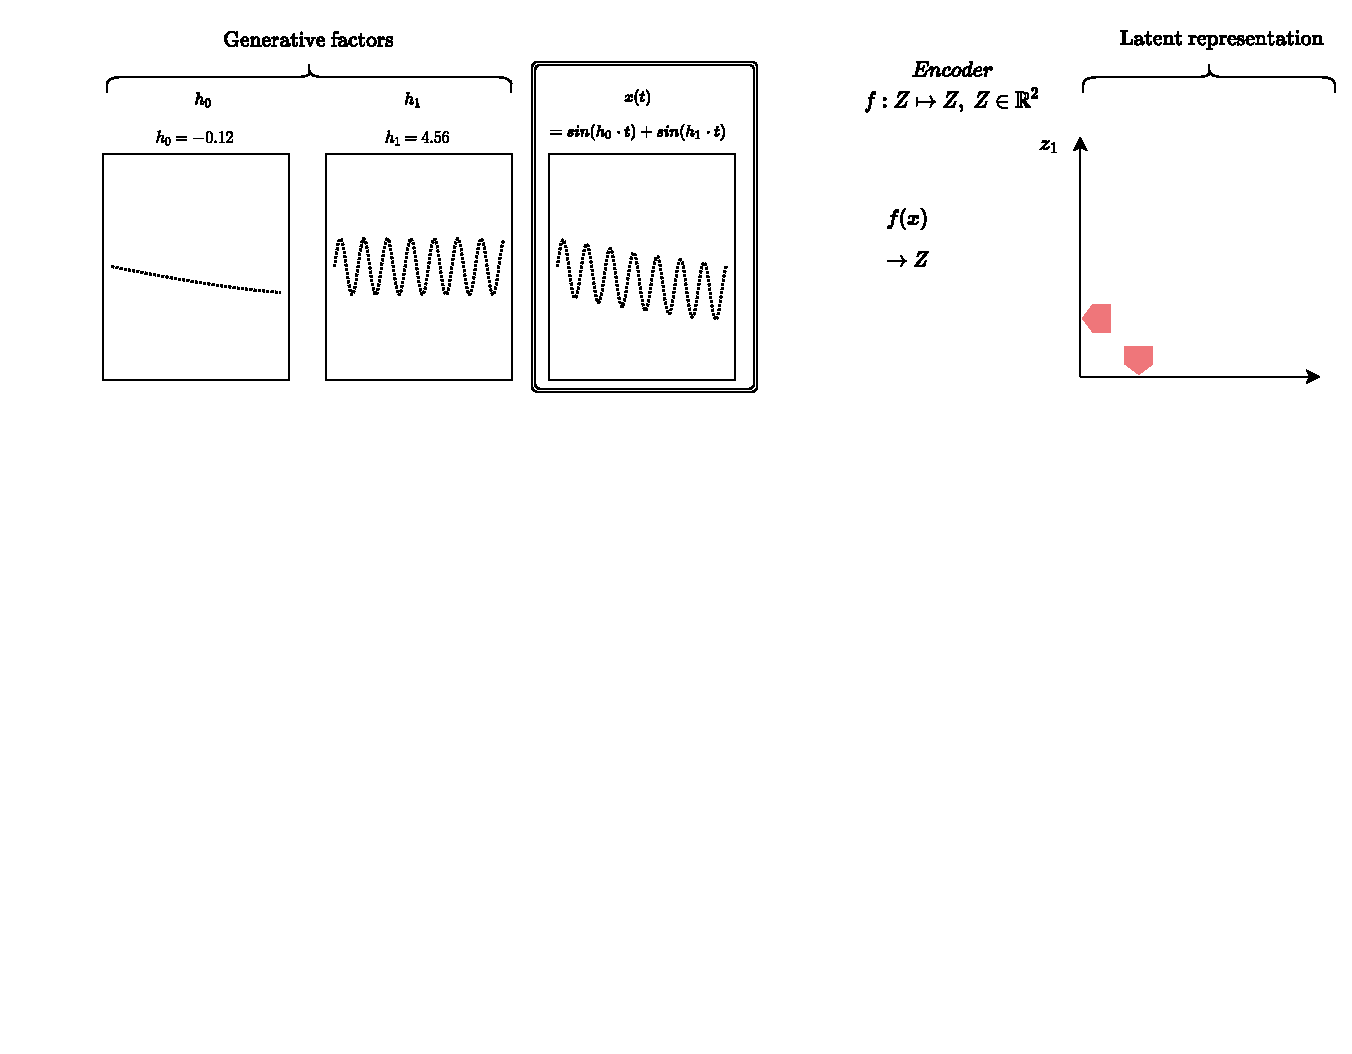
\includegraphics[width=.93\linewidth]{figures/intution_3x3_1.pdf}
	%\caption{World states are determinded by two generative factors, a change in those is reflected in the two corresponding latent variables, our $f$ maps to}
\end{figure}
\end{frame}
\setbeamercolor{background canvas}{bg=white}
\setbeamercolor{normal text}{fg=darkgrey}
\usebeamercolor[fg]{normal text}
\setbeamertemplate{itemize item}{\color{darkgrey}$\circ$}
\begin{frame}
\frametitle{What is disentanglement?}
\framesubtitle{Intuition}
\begin{itemize}%\setlength\itemsep{1.5em}
	\item Encode distinct generating factors in separate subsets of latent space dimensions
	%\item i.e. color as one subspace, translation, as another
	%\item The exact definition is often discussed, we will have a look at a proposed one
\end{itemize}
%\animategraphics[autoplay,loop,width=\linewidth/2]{10}{disentangled_scene-}{0}{19}
\begin{figure}
	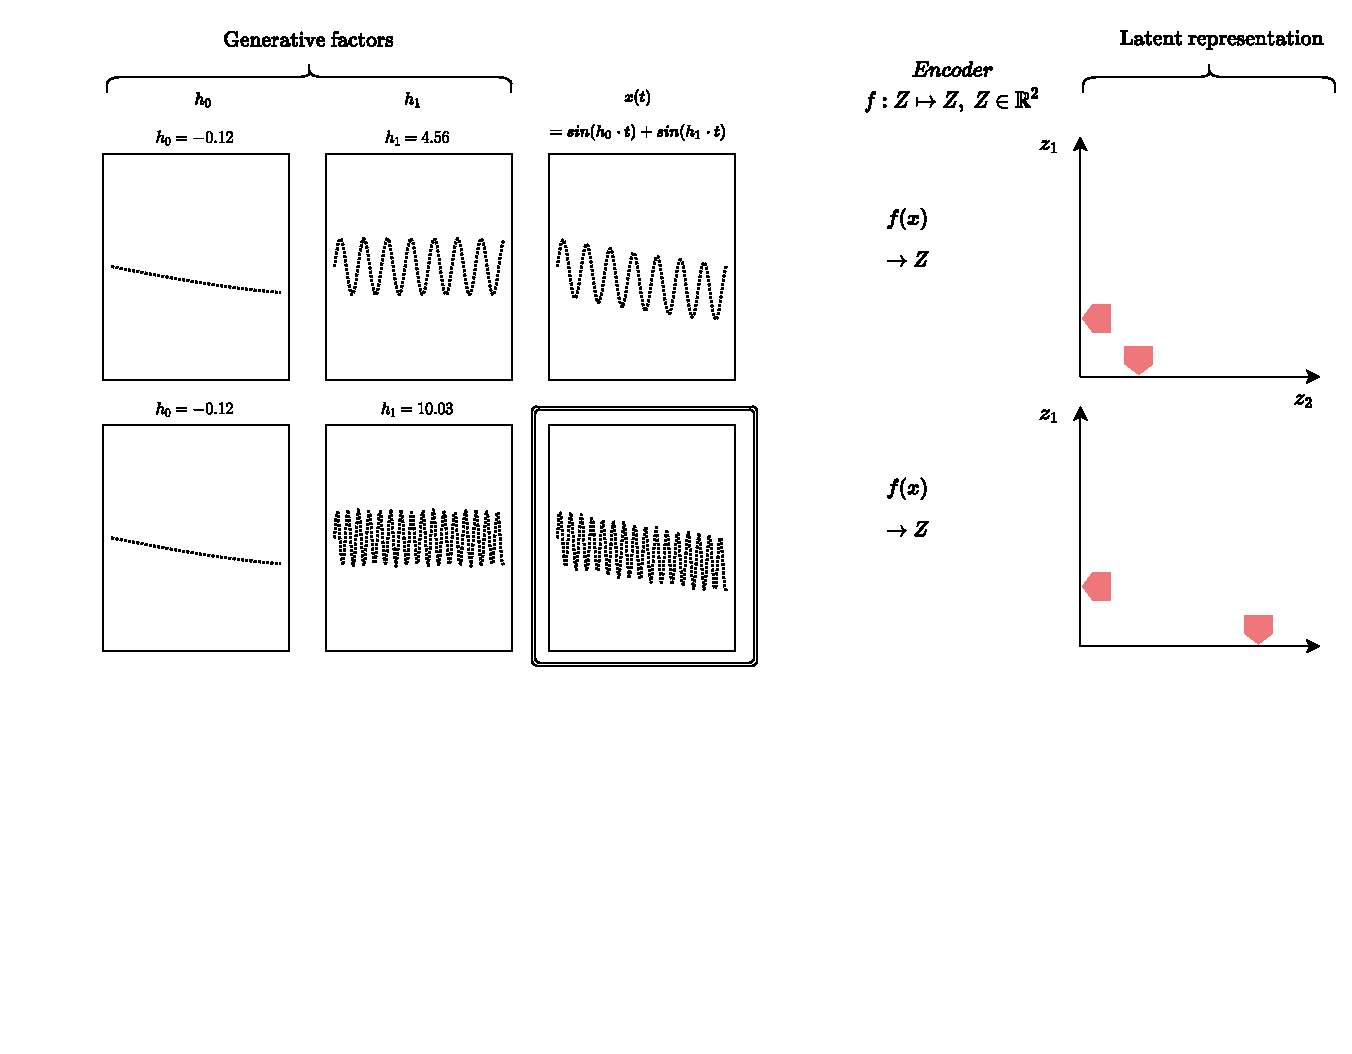
\includegraphics[width=.93\linewidth]{figures/intution_3x3_2.pdf}
	%\caption{World states are determinded by two generative factors, a change in those is reflected in the two corresponding latent variables, our $f$ maps to}
\end{figure}
\end{frame} 
\setbeamercolor{background canvas}{bg=white}
\setbeamercolor{normal text}{fg=darkgrey}
\usebeamercolor[fg]{normal text}
\setbeamertemplate{itemize item}{\color{darkgrey}$\circ$}
\begin{frame}
\frametitle{What is disentanglement?}
\framesubtitle{Intuition}
\begin{itemize}%\setlength\itemsep{1.5em}
	\item Encode distinct generating factors in separate subsets of latent space dimensions
	%\item i.e. color as one subspace, translation, as another
	%\item The exact definition is often discussed, we will have a look at a proposed one
\end{itemize}
%\animategraphics[autoplay,loop,width=\linewidth/2]{10}{disentangled_scene-}{0}{19}
\begin{figure}
	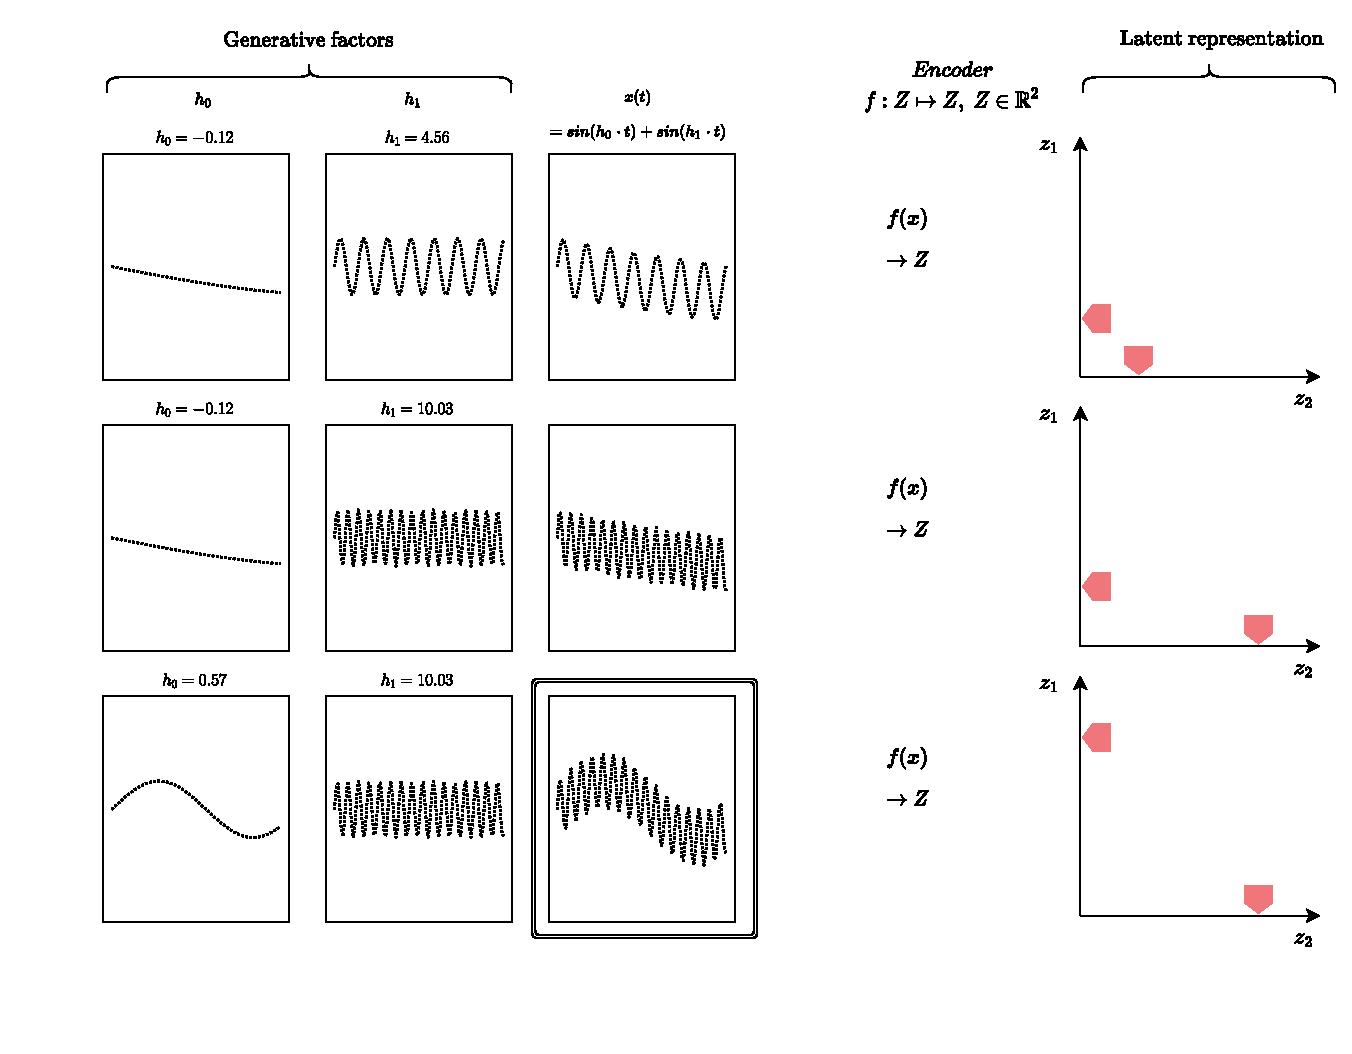
\includegraphics[width=.93\linewidth]{figures/intution_3x3_3.pdf}
	%\caption{World states are determinded by two generative factors, a change in those is reflected in the two corresponding latent variables, our $f$ maps to}
\end{figure}
\end{frame} 





\setbeamercolor{background canvas}{bg=white}
\setbeamercolor{normal text}{fg=darkgrey}
\usebeamercolor[fg]{normal text}
\setbeamertemplate{itemize item}{\color{darkgrey}$\circ$}
\begin{frame}
\frametitle{Why learn disentangled representations?}
\framesubtitle{Motivation}
\begin{itemize}%\setlength\itemsep{1.5em}
	\item Explainability/Interpretability
	\item Fairness
	\item Scientific modeling %we often know, what generating factors are, and want our model to reflect those
	\item Speaker verification %independent of content
	\item Denoising
\end{itemize}
\end{frame} 



\setbeamercolor{background canvas}{bg=white}
\setbeamercolor{normal text}{fg=darkgrey}
\usebeamercolor[fg]{normal text}
\setbeamertemplate{itemize item}{\color{darkgrey}$\circ$}
\begin{frame}
\frametitle{Disentangled Representations Formally}
\framesubtitle{A field-trip to group theory: important concepts}
\begin{itemize}%look at simple example here
	\item Group
	\begin{itemize}
		\item Operation and non-empty set $G=(\circ, G)$
		\item set closed under operation, identity element, inverses elements, associativity
	\end{itemize}
	\item Symmetry group
	\begin{itemize}
		\item Set of transformations that leave object $X$ invariant %(i.e. another set)
		\item Operation is composition of transformations
	\end{itemize}
	\item Group action
	\begin{itemize}
		\item Results of symmetry transformations on object $X$
		\item i.e. set of changed order (permuation)
		%For example permutation
	\end{itemize}
	\item Direct product
	\begin{itemize}
		\item $G = G_1 \times ... \times G_n$
		%\item Group conditions must hold for group and each subgroup
	\end{itemize}
 \end{itemize}
\end{frame} 



\setbeamercolor{background canvas}{bg=white}
\setbeamercolor{normal text}{fg=darkgrey}
\usebeamercolor[fg]{normal text}
\setbeamertemplate{itemize item}{\color{darkgrey}$\circ$}
\begin{frame}
\frametitle{Disentangled Representations Formally}
\framesubtitle{A field-trip to group theory: What is disentanglement in terms of group theory?}
\begin{itemize}%\setlength\itemsep{1.5em}
	\item Disentangled group actions
	\begin{itemize}
		\item Result of subset of symmetries $G_i$ that only change subset $X_i$ of object, but leave other $X_{j \neq i}$ invariant
	\end{itemize}
	\item $\rightarrow$ If we observe disentangled group actions in the world, we want to model those
	%G are all the symmetries of our beautiful world
	\item We can assume $G$ can be decomposed into direct product of symmetry subgroups $g_i$
\end{itemize}
\end{frame} 

\setbeamercolor{background canvas}{bg=white}
\setbeamercolor{normal text}{fg=darkgrey}
\usebeamercolor[fg]{normal text}
\setbeamertemplate{itemize item}{\color{darkgrey}$\circ$}
\begin{frame}
\frametitle{Disentangled Representations Formally}
\framesubtitle{A field-trip to group theory: What is disentanglement in terms of group theory?}
\begin{itemize}%\setlength\itemsep{1.5em}
	\item We want to find symmetry preserving mapping $f:X \mapsto Z$
	%\item Symmetry $G$ on $X$ should be preserved in $Z$%, $G \times Z \mapsto Z$
%	\begin{itemize}
%		\item $g \cdot f(x) = f(g\cdot x)$ $\rightarrow$ equivariant map
%	\end{itemize}
	\begin{align*}
		&X \;\xrightarrow[\text{}]{G}\;\;X\\ 
		f&\downarrow \;\;\;\;\;\;\;f\downarrow\\
		&Z \;\xrightarrow[\text{}]{G}\;\;\;Z
	\end{align*}
	\item $\rightarrow$ Equivariant map $g \cdot f(x) = f(g\cdot x)$
	\item Result is disentangled representation
	\begin{itemize}
		%representation reflects transformation applied to input
		\item Decomposition $Z = Z_{1} \times ... \times Z_{n}$
		\item where $Z_{i}$ is only affected by transformations $G_i$ on $X$% ($G_{j\neq i}$)
		\item and $Z_i$ invariant to all $G_{j \neq i}$ on $X$ %$Z_{warped}$ is only affected by warps in $W$ ($G_{warps}$) % G acts on W this affects Z
		\item $\rightarrow$ each subspace $Z_i$ can be transformed ONLY by the corresponding symmetry $G_i$ on $W$ (or on $Z$)%(like shift or warp independently)
		%\item We can say, $G_i$ results in disentangled group actions in $Z$
	\end{itemize}
\end{itemize}
\end{frame} 

%\setbeamercolor{background canvas}{bg=white}
%\setbeamercolor{normal text}{fg=darkgrey}
%\usebeamercolor[fg]{normal text}
%\setbeamertemplate{itemize item}{\color{darkgrey}$\circ$}
%\begin{frame}
%\frametitle{Disentangled Representations Formally}
%\framesubtitle{A field-trip to group theory: What is disentanglement in terms of group theory?}
%\begin{itemize}%\setlength\itemsep{1.5em}
%	\item Representation is disentangled if:
		%\item action $\cdot : G \times Z \mapsto Z$
%		\item equivariant map $f:X \mapsto Z$%, g \cdot f(w) = f(g\cdot w) \forall g \in G,w \in W$ % %between actions on $W$ and $Z$
%		\item such a map would split $Z$ into independent subspaces, thus satisfying:
%		\begin{itemize}
			%representation reflects transformation applied to input
%			\item Decomposition $Z = Z_{1} \times ... \times Z_{n}$
%			\item where $Z_{i}$ is only affected by transformations $G_i$ in $W$% ($G_{j\neq i}$)
%			\item and $Z_i$ invariant to all $G_{j \neq i}$ in $W$ %$Z_{warped}$ is only affected by warps in $W$ ($G_{warps}$) % G acts on W this affects Z
%			\item Thus each subspace $Z_i$ can be transformed ONLY by the corresponding symmetry $G_i$ on $W$ (or on $Z$)%(like shift or warp independently)
			%\item We can say, $G_i$ results in disentangled group actions in $Z$
%		\end{itemize}
		%\item action $\cdot$ on $Z$ is disentangled according to definition from before
	%\item There may be more criteria (preserving group structure, isomorphisms, ...) but for the intuition this is sufficient
	%\item (Note that much prior knowledge about our world was injected here)
%\end{itemize}
%\end{frame} 



%\setbeamercolor{background canvas}{bg=white}
%\setbeamercolor{normal text}{fg=darkgrey}
%\usebeamercolor[fg]{normal text}
%\setbeamertemplate{itemize item}{\color{darkgrey}$\circ$}
%\begin{frame}
%\frametitle{Disentangled Representations Formally}
%\framesubtitle{A field-trip to group theory: Disentangle our example formally}
%\begin{itemize}%\setlength\itemsep{1.5em}
%	\item signal $x(t) = sin(h_0 \cdot t) + sin(h_1 \cdot t)$ with $h_0 \sim \mathcal{N}(0,1),\;h_1 \sim \mathcal{N}(5,1);$
%	\item The set of possible values for $h_0, h_1$ make up our $W$
%	\item The group of symmetries acting on this $W$ decompose into $G = G_{h_0} \times G_{h_1}$
%	\item We want to find an equivariant map $f:W\mapsto Z$ with $Z \in \mathbb{Z}^2$
%	\item so that changes of $h_0$ result ONLY in changes in $z_0$ and changes of $h_1$ ONLY in $z_2$
%	\item Note, that this requires prior knowledge of generating factors in our world
%\end{itemize}
%\end{frame} 





\setbeamercolor{background canvas}{bg=white}
\setbeamercolor{normal text}{fg=darkgrey}
\usebeamercolor[fg]{normal text}
\setbeamertemplate{itemize item}{\color{darkgrey}$\circ$}
\begin{frame}
\frametitle{Back to the paper}
\framesubtitle{Did they achieve disentanglement?}
\begin{itemize}
	\item Disentangled with respect to what decomposition?
	\item Assume decomposition $G = G_{sequence} \times G_{segment}$
	\item Reflect decomposition in $Z= (z_1, z_2)$
	\item $z_1$: segment, $z_2$: sequence
	%\item They propose to store sequence information in $z_2$ and segment information in $z_1$
	\item Find equivariant map $f:W\mapsto Z$, so that $z_2$ is only affected by actions of $G_{sequence}$ and vice versa
\end{itemize}
\begin{figure}
	\includegraphics[width=.9\linewidth]{figures/fm_variables.png}
\end{figure}
\begin{tiny}
	Image source: Hsu et al., 2017 
\end{tiny}
\end{frame} 



\setbeamercolor{background canvas}{bg=white}
\setbeamercolor{normal text}{fg=darkgrey}
\usebeamercolor[fg]{normal text}
\setbeamertemplate{itemize item}{\color{darkgrey}$\circ$}
\begin{frame}
\frametitle{FHVAE}
\framesubtitle{Encoder$_{\theta}$}
\begin{figure}
	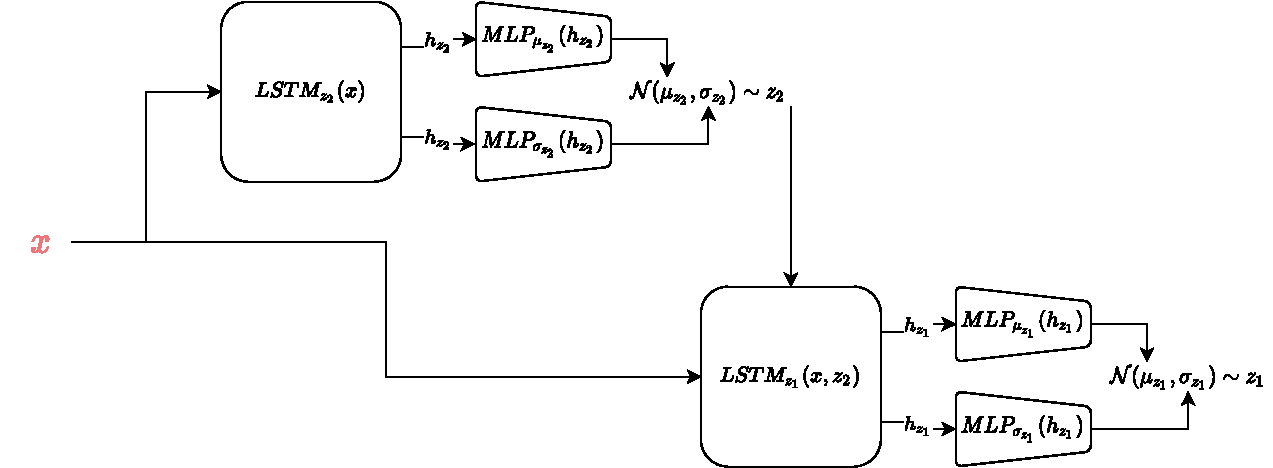
\includegraphics[width=1.05\linewidth]{figures/fhvae_decoder_0.pdf}
\end{figure}
\end{frame}
\setbeamercolor{background canvas}{bg=white}
\setbeamercolor{normal text}{fg=darkgrey}
\usebeamercolor[fg]{normal text}
\setbeamertemplate{itemize item}{\color{darkgrey}$\circ$}
\begin{frame}
\frametitle{FHVAE}
\framesubtitle{Encoder$_{\theta}$}
\begin{figure}
	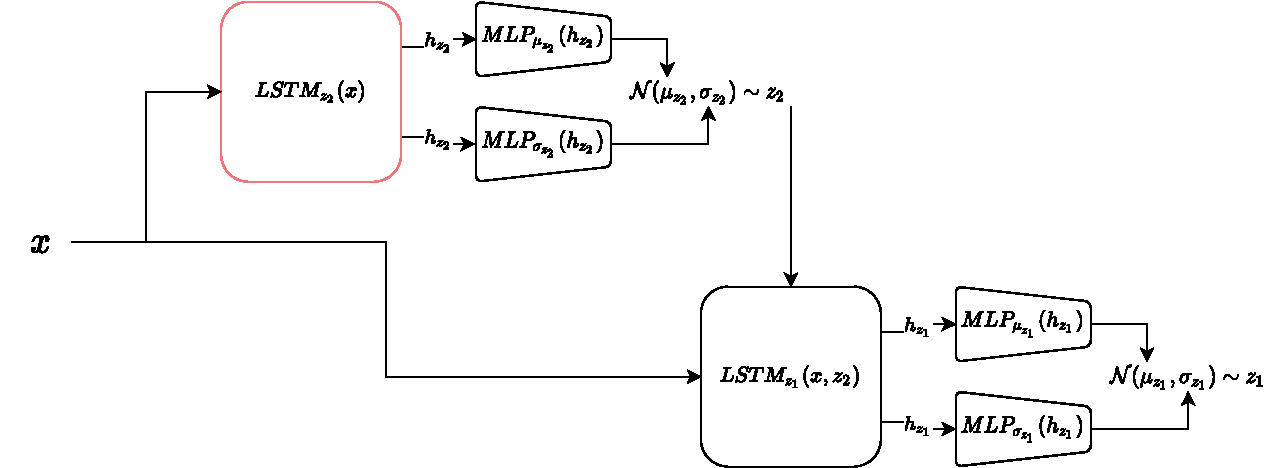
\includegraphics[width=1.05\linewidth]{figures/fhvae_decoder_1.pdf}
\end{figure}
\end{frame} 
\setbeamercolor{background canvas}{bg=white}
\setbeamercolor{normal text}{fg=darkgrey}
\usebeamercolor[fg]{normal text}
\setbeamertemplate{itemize item}{\color{darkgrey}$\circ$}
\begin{frame}
\frametitle{FHVAE}
\framesubtitle{Encoder$_{\theta}$}
\begin{figure}
	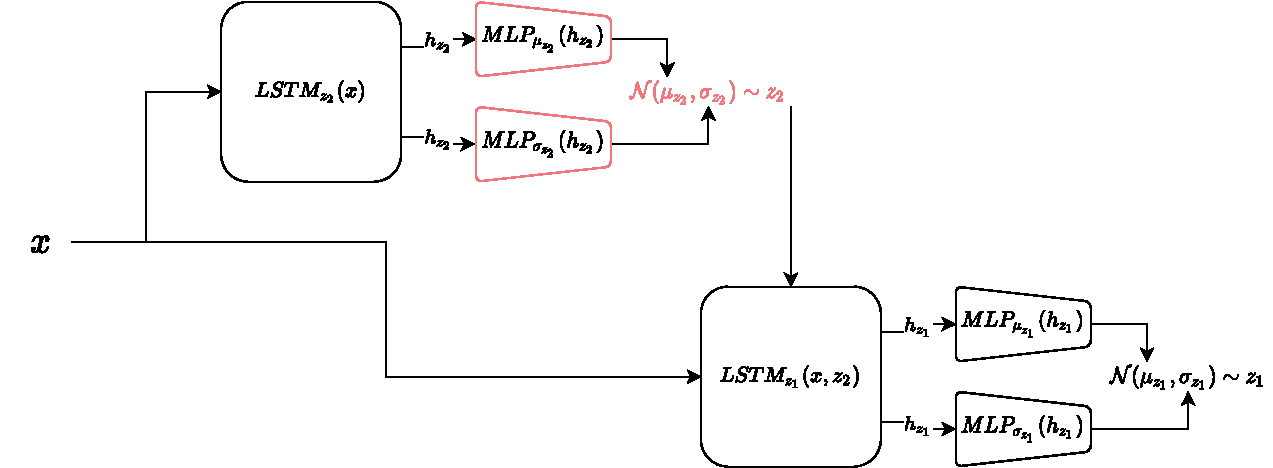
\includegraphics[width=1.05\linewidth]{figures/fhvae_decoder_2.pdf}
\end{figure}
\end{frame} 
\setbeamercolor{background canvas}{bg=white}
\setbeamercolor{normal text}{fg=darkgrey}
\usebeamercolor[fg]{normal text}
\setbeamertemplate{itemize item}{\color{darkgrey}$\circ$}
\begin{frame}
\frametitle{FHVAE}
\framesubtitle{Encoder$_{\theta}$}
\begin{figure}
	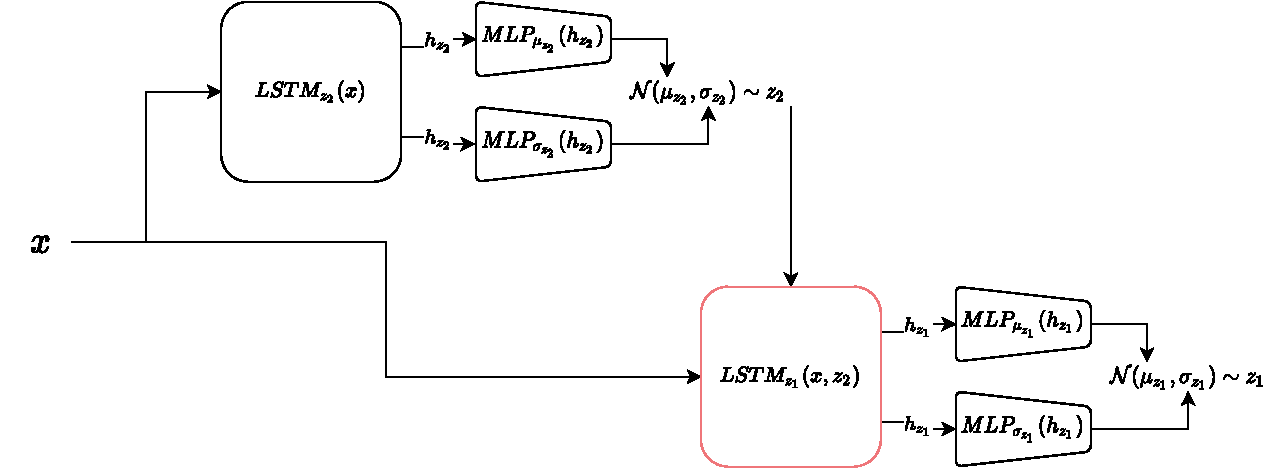
\includegraphics[width=1.05\linewidth]{figures/fhvae_decoder_3.pdf}
\end{figure}
\end{frame} 
\setbeamercolor{background canvas}{bg=white}
\setbeamercolor{normal text}{fg=darkgrey}
\usebeamercolor[fg]{normal text}
\setbeamertemplate{itemize item}{\color{darkgrey}$\circ$}
\begin{frame}
\frametitle{FHVAE}
\framesubtitle{Encoder$_{\theta}$}
\begin{figure}
	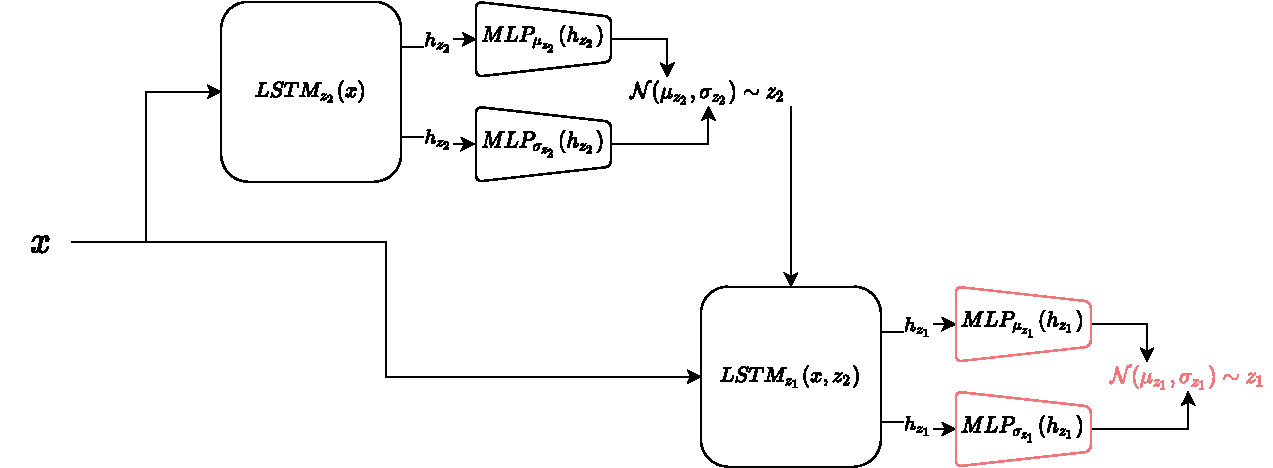
\includegraphics[width=1.05\linewidth]{figures/fhvae_decoder_4.pdf}
\end{figure}
\end{frame} 
\setbeamercolor{background canvas}{bg=white}
\setbeamercolor{normal text}{fg=darkgrey}
\usebeamercolor[fg]{normal text}
\setbeamertemplate{itemize item}{\color{darkgrey}$\circ$}
\begin{frame}
\frametitle{FHVAE}
\framesubtitle{Decoder$_{\phi}$}
\begin{figure}
	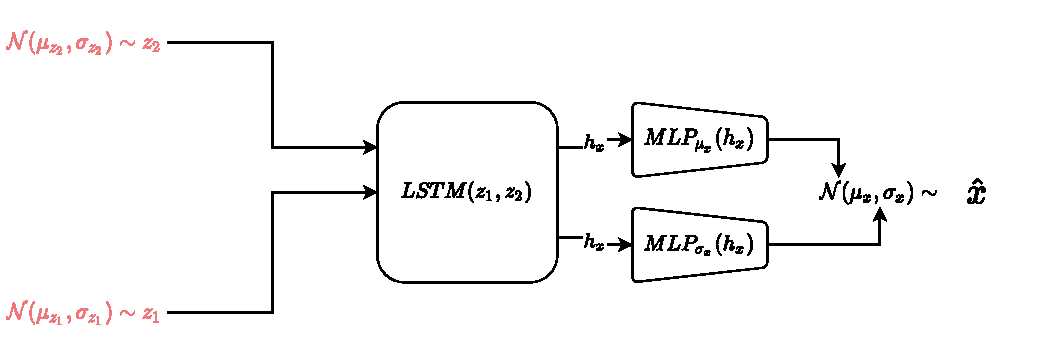
\includegraphics[width=1.05\linewidth]{figures/fhvae_encoder_0.pdf}
\end{figure}
\end{frame} 
\setbeamercolor{background canvas}{bg=white}
\setbeamercolor{normal text}{fg=darkgrey}
\usebeamercolor[fg]{normal text}
\setbeamertemplate{itemize item}{\color{darkgrey}$\circ$}
\begin{frame}
\frametitle{FHVAE}
\framesubtitle{Decoder$_{\phi}$}
\begin{figure}
	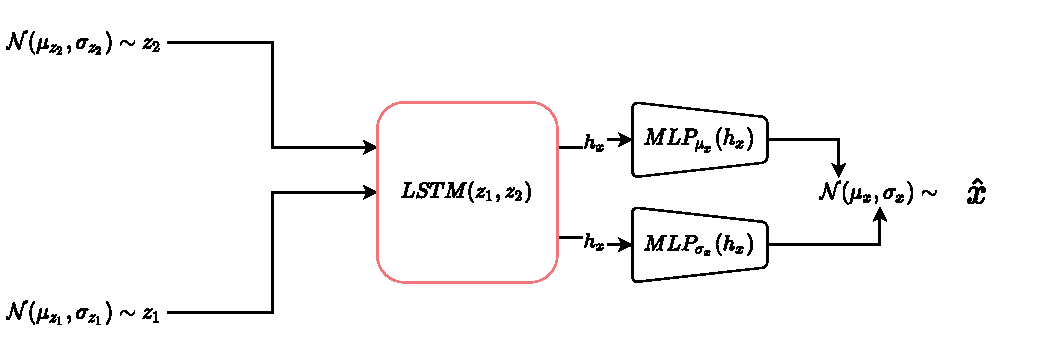
\includegraphics[width=1.05\linewidth]{figures/fhvae_encoder_1.pdf}
\end{figure}
\end{frame} 
\setbeamercolor{background canvas}{bg=white}
\setbeamercolor{normal text}{fg=darkgrey}
\usebeamercolor[fg]{normal text}
\setbeamertemplate{itemize item}{\color{darkgrey}$\circ$}
\begin{frame}
\frametitle{FHVAE}
\framesubtitle{Decoder$_{\phi}$}
\begin{figure}
	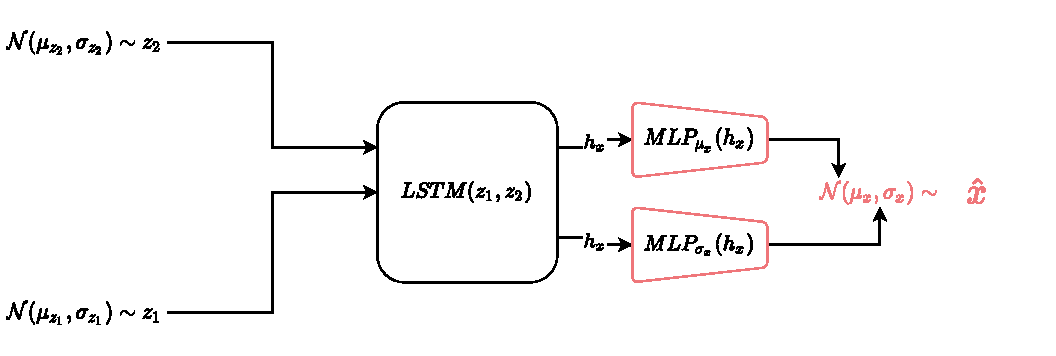
\includegraphics[width=1.05\linewidth]{figures/fhvae_encoder_2.pdf}
\end{figure}
\end{frame} 





\setbeamercolor{background canvas}{bg=white}
\setbeamercolor{normal text}{fg=darkgrey}
\usebeamercolor[fg]{normal text}
\setbeamertemplate{itemize item}{\color{darkgrey}$\circ$}
\begin{frame}
\frametitle{FHVAE}
\framesubtitle{Objective}
%\begin{itemize}
%	\item regularize $z_1$ globally (through standard Gaussian prior)
%	\item regularize $z_2$ through sequence dependent prior $\tilde{\mu_2}$
%\end{itemize}
\begin{align*}
\mathcal{L}(\theta, \phi, X)& = \sum_{n=1}^N \color{sienna}\underbrace{\mathcal{L}(\theta, \phi;x^{(n)}|\tilde{\mu_2}) \color{black}+\color{black} log\;p_{\theta}(\tilde{\mu_2})\color{black} + const.}_{\text{var. lower bound}} + \color{cornflower}\underbrace{\color{black}\alpha \cdot \color{cornflower}log\;(i|z_2^{(i,n)})}_{\text{discrim.obj.}}\\
\text{with }\color{sienna}\mathcal{L}(\theta, \phi;x^{(n)}|\tilde{\mu_2}) &\color{sienna}= \mathbb{E}_{q_{\phi}(z_1^{(n)},z_2^{(n)}|x^{(n)})}\left[ log\;p_{\theta}(x^{(n)}|z_1^{(n)},z_2^{(n)}) \right]\\
-& \color{sienna}\mathbb{E}_{q_{\phi}(z_2^{(n)}|x^{(n)})} \left[ D_{KL}(q_{\phi}(z_1^{(n)}|x^{(n)},z_2^{(n)}) ||\underbrace{p_{\theta}(z_1^{(n)})}_{\text{sequ. ind.}}) \right]\\
-&\color{sienna}D_{KL}(q_{\phi}(z_2^{(n)}|x^{(n)})||\underbrace{p_{\theta}(z_2^{(n)}|\tilde{\mu_2})}_{\text{seq. dep. prior}})\\
\color{black}\text{and }\color{cornflower}log\;(i|z_2^{(i,n)}) &=\color{cornflower} log\;p(z_{2}^{(i,n)}|\tilde{\mu_2}^{(i)}) - log(\sum_{j=1}^{M}p(z_2^{(i,n)}|\mu_2^{(j)}))
\end{align*}
\end{frame} 


\setbeamercolor{background canvas}{bg=white}
\setbeamercolor{normal text}{fg=darkgrey}
\usebeamercolor[fg]{normal text}
\setbeamertemplate{itemize item}{\color{darkgrey}$\circ$}
\begin{frame}
\frametitle{FHVAE}
\framesubtitle{S-vector $\mu_2$}
\begin{itemize}
	\item What is sequence dependent prior $\mu_2$ (s-vector)?
	\begin{itemize}
		\item imagine a word vector 
		\item s-vector for every sequence
		\item similar sequence $\rightarrow$ in s-vectors close in euclidean space
		%\item Ideally, similarities in sequences should  result in s-vectors close in euclidian space
		\item $g(sequence\;id) = \mu_2$ as differentiable lookup table
		\begin{itemize}
			\item $\rightarrow$ embedding in pytorch, tensorflow
		\end{itemize}
		%\item During test, s-vector can be found in closed form solution %where there is no seq.id available
	\end{itemize}
\end{itemize}
\end{frame} 



\setbeamercolor{background canvas}{bg=white}
\setbeamercolor{normal text}{fg=darkgrey}
\usebeamercolor[fg]{normal text}
\setbeamertemplate{itemize item}{\color{darkgrey}$\circ$}
\begin{frame}
\frametitle{FHVAE}
\framesubtitle{Objective - Sequence variational lower bound}
\begin{align*}
\mathcal{L}(\theta, \phi, X)& = %\sum_{n=1}^N \mathcal{L}(\theta, \phi;x^{(n)}|\tilde{\mu_2}) + log\;p_{\theta} + const.\\
%\mathcal{L}(\theta, \phi;x^{(n)}|\tilde{\mu_2}) &= 
\underbrace{log\;p(x|z_1, z_2)}_{\text{reconstruction}}\\%prob. of obs. data under learned posterior\\
-&\underbrace{D_{KL}(\mathcal{N}(\mu_{z_1}, \sigma_{z_1})||\mathcal{N}(0,1))}_{\text{regularize $z_1$ with global prior}}\\
-&\underbrace{D_{KL}(\mathcal{N}(\mu_{z_2}, \sigma_{z_2})||\mathcal{N}(\tilde{\mu_2},0.5))}_{\text{regularize $z_2$ with seq. dep. prior $\mu_2$}}\\
+&\underbrace{log\;p(\tilde{\mu_2}) \cdot \frac{1}{seq.\;length}}_{\text{prob. of $\tilde{\mu_2}$ under standard Gaussian prior}}
\end{align*}
\end{frame} 



\setbeamercolor{background canvas}{bg=white}
\setbeamercolor{normal text}{fg=darkgrey}
\usebeamercolor[fg]{normal text}
\setbeamertemplate{itemize item}{\color{darkgrey}$\circ$}
\begin{frame}
\frametitle{FHVAE}
\framesubtitle{Objective - Discriminative objective}
\begin{align*}
log\;p(sequence\;id | z_2)& = CrossEntropy(\frac{-(\mu_{z_2} - \mu_2)^2}{\sigma_{z_2}^2},\;sequence\;id)
\end{align*}
\begin{itemize}
	\item $\rightarrow$ Try to predict sequence id with $z_2$
\end{itemize}
\end{frame} 



\setbeamercolor{background canvas}{bg=white}
\setbeamercolor{normal text}{fg=darkgrey}
\usebeamercolor[fg]{normal text}
\setbeamertemplate{itemize item}{\color{darkgrey}$\circ$}
\begin{frame}
\frametitle{FHVAE}
\framesubtitle{Objective - Discriminative segment variational lower bound}
\begin{align*}
\mathcal{L}^{dis}(\theta, \phi;x)& = \mathcal{L}(\theta, \phi, X) + \alpha \cdot log\;p(sequence\;id | z_2)
\end{align*}
\begin{itemize}
	\item Joint objective
	\begin{itemize}
		\item encourage factorization
	\end{itemize}
	\item discriminative objective can be adjusted through $\alpha$ hyperparameter
	\begin{itemize}
		\item encourage $\mu_{z_2}$ to become more meaningful
	\end{itemize}
\end{itemize}
\end{frame} 

%\setbeamercolor{background canvas}{bg=white}
%\setbeamercolor{normal text}{fg=darkgrey}
%\usebeamercolor[fg]{normal text}
%\setbeamertemplate{itemize item}{\color{darkgrey}$\circ$}
%\begin{frame}
%\frametitle{FHVAE}
%\framesubtitle{Short recap}
%\begin{itemize}
	%\item We want to disentangle sequential data with respect to sequence and segment variables
%	\item We do this by learning two latent variables $z_1$ and $z_2$ with FHVAE
%	\item Disentanglement between the two is encouraged through loss term%an adaptive regularization
%	\item Now, we want to see, whether it worked
%\end{itemize}
%\end{frame} 










\setbeamercolor{background canvas}{bg=white}
\setbeamercolor{normal text}{fg=darkgrey}
\usebeamercolor[fg]{normal text}
\setbeamertemplate{itemize item}{\color{darkgrey}$\circ$}
\begin{frame}
\frametitle{FHVAE}
\framesubtitle{Results - TIMIT Speaker Verification} % Maybe rather do ASR here
\begin{itemize}
	\item Task: Speaker verification
	\begin{itemize}
		\item Allows quantitative analysis of performance
		\item Assess quality of disentanglement
		\item Use s-vector $\mu_2$ to predict speaker
	\end{itemize}
	\item Compare i-vector baseline
	\begin{itemize}
		\item i-vector used in SOTA speaker verification approaches
		\item Low dimensional subspace of GMM universal background model
		\item Contains speaker information (content-independent)
		%\item contain sequence level info (-> speaker)
		%\item Sequence features from this GMM
	\end{itemize}
\end{itemize}
\end{frame} 


\setbeamercolor{background canvas}{bg=white}
\setbeamercolor{normal text}{fg=darkgrey}
\usebeamercolor[fg]{normal text}
\setbeamertemplate{itemize item}{\color{darkgrey}$\circ$}
\begin{frame}
\frametitle{FHVAE}
\framesubtitle{Results - TIMIT Speaker Verification} % Maybe rather do ASR here
\begin{itemize}
	\item Unsupervised speaker verification (Raw column)
	\item Metric: equal error rate (lower is better)
	\item $\mu_1$ based on $z_1$ as sanity check
\end{itemize}
\begin{figure}
	\includegraphics[width=.8\linewidth]{figures/timit_error.png}
	%\caption{Comparison of speaker verification equal error rate (EER) on TIMIT dataset (lower is better)}
	%\caption{World states are determinded by two generative factors, a change in those is reflected in the two corresponding latent variables, our $f$ maps to}
\end{figure}
\end{frame} 



\setbeamercolor{background canvas}{bg=white}
\setbeamercolor{normal text}{fg=darkgrey}
\usebeamercolor[fg]{normal text}
\setbeamertemplate{itemize item}{\color{darkgrey}$\circ$}
\begin{frame}
\frametitle{FHVAE}
\framesubtitle{Looking Back \& Discussion} % Maybe rather do ASR here
\begin{itemize}
	\item Evidence towards disentangling with respect to sequence-segment decomposition
	\begin{itemize}
		\item other decompositions may prove more challenging
		%\item speaker gender, speaker age, language as more fine grained decompositions
	\end{itemize}
	\item Good performance on speaker verification and denoising task
	\item I had trouble disentangling simple examples
	\item Questions for you
	\begin{itemize}
		\item Is learning disentangled representations worth the effort?
		\item Have there been situations where you wished for an interpretable latent space?
		\item Do you know any successful models where equivariant maps are used?
		%\item Are there any models you know, which use disentangled representations (with respect to some decomposition)
	\end{itemize}
\end{itemize}
\end{frame} 


\setbeamercolor{background canvas}{bg=white}
\setbeamercolor{normal text}{fg=darkgrey}
\usebeamercolor[fg]{normal text}
\setbeamertemplate{itemize item}{\color{darkgrey}$\circ$}
\begin{frame}
\frametitle{References}
\framesubtitle{}
\begin{itemize}
	\item Hsu, W.N., Zhang, Y. and Glass, J., 2017. Unsupervised learning of disentangled and interpretable representations from sequential data. In Advances in neural information processing systems (pp. 1878-1889).
	\item Higgins, I., Amos, D., Pfau, D., Racaniere, S., Matthey, L., Rezende, D. and Lerchner, A., 2018. Towards a definition of disentangled representations. arXiv preprint arXiv:1812.02230.
	\item Scott, W.R., 2012. Group theory. Courier Corporation.
	\item Kingma, D.P. and Welling, M., 2013. Auto-encoding variational bayes. arXiv preprint arXiv:1312.6114.
\end{itemize}
\end{frame} 




\setbeamercolor{background canvas}{bg=white}
\setbeamercolor{normal text}{fg=darkgrey}
\usebeamercolor[fg]{normal text}
\setbeamertemplate{itemize item}{\color{darkgrey}$\circ$}
\begin{frame}
\frametitle{}
\framesubtitle{}
\begin{itemize}
	\item 
\end{itemize}
\end{frame} 


\setbeamercolor{background canvas}{bg=white}
\setbeamercolor{normal text}{fg=darkgrey}
\usebeamercolor[fg]{normal text}
\setbeamertemplate{itemize item}{\color{darkgrey}$\circ$}
\begin{frame}
\frametitle{Disentangled Representations Formally}
\framesubtitle{A field-trip to group theory: Disentangle our example formally}
\begin{itemize}%\setlength\itemsep{1.5em}
	\item Signal can get shifted or warped
	\item the set of these transformations make up a symmetry group
	\item This can be decomposed into shifts and warps/subsets of original set (all shifted $\times$ all warped)
	%\item signal's meaning is preserved
	\item Either content is preserved, or speaker is preserved
	\item the resulting set of transformed signals are the actions of the symmetry group on the world state
\end{itemize}
\end{frame} 

%%%%%%%%%%%%%%%%%%%%%%%%%%%%%%%%%%%%%%%%%%%%%%%%%%%%%%



\setbeamercolor{background canvas}{bg=white}
\setbeamercolor{normal text}{fg=darkgrey}
\usebeamercolor[fg]{normal text}
\setbeamertemplate{itemize item}{\color{darkgrey}$\circ$}
\begin{frame}
\frametitle{Disentangled Representations Formally}
\framesubtitle{A field-trip to group theory}
\begin{itemize}%\setlength\itemsep{1.5em}
	\item This symmetry group can be decomposed into symmetry subgroups
	\item One affects location
	\item the other affects frequence
\end{itemize}
\end{frame} 

\setbeamercolor{background canvas}{bg=white}
\setbeamercolor{normal text}{fg=darkgrey}
\usebeamercolor[fg]{normal text}
\setbeamertemplate{itemize item}{\color{darkgrey}$\circ$}
\begin{frame}
\frametitle{What are disentangled representations formally? }
\framesubtitle{Disentangled Group Action}
\begin{itemize}%\setlength\itemsep{1.5em}
	\item Group action $G \times X \mapsto X$
	\item Group decomposes into direct product $G = G_{shifts} \times G_{warps}$
	\item Is disentangled with respect to decomposition of $G$
	\begin{itemize}
		\item if there is decomposition $X = X_{shifted} \times X_{warped}$
		\item and actions $G_{shifts} \times X_{shifted} \mapsto X_{shifted}$
		\item and actions $G_{warps} \times X_{warped} \mapsto X_{warped}$
	\end{itemize}
\end{itemize}
\end{frame} 

\setbeamercolor{background canvas}{bg=white}
\setbeamercolor{normal text}{fg=darkgrey}
\usebeamercolor[fg]{normal text}
\setbeamertemplate{itemize item}{\color{darkgrey}$\circ$}
\begin{frame}
\frametitle{What are disentangled representations formally? }
\framesubtitle{Disentangled Representation}
\begin{itemize}%\setlength\itemsep{1.5em}
	\item Let $W$ be the set of world states (all shifts and warps of signal)
	\item Generative process $b:W \mapsto O$ (voice to audio processing unit)
	\item Inference process $h: O \mapsto Z$ (observation to latent space)
	\item $f:W \mapsto Z, f = h \circ b$
	\item Now, we know, there is a symmetry group acting on $W$ ($G \times W \mapsto W$)
	\item We want to find corresponding $G \times Z \mapsto Z$ to reflect symmetry structure of W in Z
	\item More formal: $g \cdot f(w) = f(g\cdot w)$
	\item This is whats called an equivariant map (famous example: convnet)
\end{itemize}
\end{frame} 



\setbeamercolor{background canvas}{bg=white}
\setbeamercolor{normal text}{fg=darkgrey}
\usebeamercolor[fg]{normal text}
\setbeamertemplate{itemize item}{\color{darkgrey}$\circ$}
\begin{frame}
\frametitle{What are disentangled representations formally? }
\framesubtitle{Disentangled Representation}
\begin{itemize}%\setlength\itemsep{1.5em}
	\item Assume symmetry transformations $G$ of $W$ decompose into direct product $G = G_1 \times ... \times G_n$
	\item Representation is disentangled if
	\begin{itemize}
		%\item action $\cdot : G \times Z \mapsto Z$
		\item equivariant map $f:W \mapsto Z, g \cdot f(w) = f(g\cdot w) \forall g \in G,w \in W$ % %between  $W$ and $Z$
		\item such a map would split $Z$ into independent subspaces, thus satisfying:
		\begin{itemize}
					%representation reflects transformation applied to input
			\item Decomposition $Z = Z_{shifted} \times Z_{warped}$
			\item where $Z_{shifted}$ is only affected by shifts in $W$ ($G_{shifts}$)
			\item and $Z_{warped}$ is only affected by warps in $W$ ($G_{warps}$) % G acts on W this affects Z
			\item Thus each subspace can be transformed by the corresponding symmetry (like shift or warp independently)
		\end{itemize}
				%\item action $\cdot$ on $Z$ is disentangled according to definition from before
	\end{itemize}
	\item There may be more criteria (preserving group structure, isomorphisms, ...) but for the intuition this is sufficient
	%\item (Note that much prior knowledge about our world was injected here)
\end{itemize}
\end{frame} 




\setbeamercolor{background canvas}{bg=white}
\setbeamercolor{normal text}{fg=darkgrey}
\usebeamercolor[fg]{normal text}
\setbeamertemplate{itemize item}{\color{darkgrey}$\circ$}
\begin{frame}
\frametitle{Did they achieve disentanglement}
\framesubtitle{...}
\begin{itemize}%\setlength\itemsep{1.5em}
	\item With respect to a decomposition into two
	\item Setting: 10 sentences, 630 speakers
	\item How can we formulate this in group theory terms?
\end{itemize}
\end{frame} 







\setbeamercolor{background canvas}{bg=white}
\setbeamercolor{normal text}{fg=darkgrey}
\usebeamercolor[fg]{normal text}
\setbeamertemplate{itemize item}{\color{darkgrey}$\circ$}
\begin{frame}
\frametitle{How did they do it?}
\framesubtitle{Intuition}
\begin{itemize}%\setlength\itemsep{1.5em}
	\item With respect to a decomposition into two
	\item regularize z2 by sequence dependant prior (lookup table of s-vectors)
	\item and z1 by sequence independant prior
\end{itemize}
\end{frame} 





\setbeamercolor{background canvas}{bg=white}
\setbeamercolor{normal text}{fg=darkgrey}
\usebeamercolor[fg]{normal text}
\setbeamertemplate{itemize item}{\color{darkgrey}$\circ$}
\begin{frame}
\frametitle{How did they do it?}
\framesubtitle{Methods}
\begin{itemize}%\setlength\itemsep{1.5em}
	\item Sample batch at segment level (instead of sequence level)
	\item Maximize segment variational lower bound
	\item (Force z2 to be close to mu2)
	\item approximation of mu2 is closed form equation (concave function, set derivative to 0)
\end{itemize}
\end{frame} 



\setbeamercolor{background canvas}{bg=white}
\setbeamercolor{normal text}{fg=darkgrey}
\usebeamercolor[fg]{normal text}
\setbeamertemplate{itemize item}{\color{darkgrey}$\circ$}
\begin{frame}
\frametitle{Challenges}
\framesubtitle{...}
\begin{itemize}%\setlength\itemsep{1.5em}
	\item If we really think about it, it is hard for us to define what a disentangled representation should actually be
	\item Precise biases of what the latent space should be decomposited into can be helpful as well as biases towards the 'form' of these latent subspaces
\end{itemize}
\end{frame} 

\end{document}
